\documentclass[11pt]{article}
\title{Meccano triangles}
\author{https://github.com/heptagons/meccano/nest}
\date{}

\newfam\bbbfam
\font\bbbten=msbm10
\font\bbbseven=msbm7
\font\bbbfive=msbm5
\textfont\bbbfam=\bbbten
\scriptfont\bbbfam=\bbbseven
\scriptscriptfont\bbbfam=\bbbfive
\def\bbb{\fam=\bbbfam}

\usepackage{../../meccano}
\usepackage{longtable}
\begin{document}

\maketitle
\begin{abstract}
We construct meccano triangles. Basic triangles has the three sides as integers and calculate the internal diagonal distances.
Such diagonals then are used as the new side of more complicated triangles and then again we
calculate new distances formed and so on. Eventually we expect to
find certain angles joining the triangles which can be used to construct regular polygons or more figures.
\end{abstract}

\section{Triangles $(a,b,c)$}
Triangles $(a,b,c)$ have three sides $a$, $b$ and $c$ where $a, b, c \in \bbb N$.
To avoid repetitions and get only valid triangles, we consider only the cases:
\begin{align}
a &\ge b \ge c\\
a &< b + c
\end{align}

The cosines of the three angles of triangle$(a,b,c)$ are rationals $\cos{A}, \cos{B}, \cos{C} \in \bbb {Q}$:
\begin{equation}\label{Eq:cosABC}
\cos\left({\begin{array}{c} A\\ B\\ C\\ \end{array}}\right)
= \left({\begin{array}{c}
\dfrac{b^2 + c^2 - a^2}{2bc}\\[10pt]
\dfrac{c^2 + a^2 - b^2}{2ca}\\[10pt]
\dfrac{a^2 + b^2 - c^2}{2ab}\\[10pt]
\end{array}}\right)
\equiv \left({\begin{array}{c}
\dfrac{a_n}{a_d}\\[10pt]
\dfrac{b_n}{b_d}\\[10pt]
\dfrac{c_n}{c_d}\\[10pt]
\end{array}}\right) \in \bbb {Q}
\end{equation}
Where numerators are integers $a_n, b_n, c_n \in \bbb{Z}$ and denominators are naturals
$a_d, b_d, c_d \in \bbb{N}$ and always $x_n <= x_d$ for $x=\{a,b,c\}$.

The sines of the three angles are algebraic $\sin{A}, \sin{B}, \sin{C} \in \bbb {A}$:
\begin{equation}\label{Eq:sinABC}
\sin\left({\begin{array}{c} A\\ B\\ C\\ \end{array}}\right)
= \left({\begin{array}{c}
\sqrt{1 - \cos^2{A}}\\[4pt]
\sqrt{1 - \cos^2{B}}\\[4pt]
\sqrt{1 - \cos^2{C}}\\[4pt]
\end{array}}\right)
= \left({\begin{array}{c}
\dfrac{\sqrt{a_d^2 - a_n^2}}{a_d}\\[10pt]
\dfrac{\sqrt{b_d^2 - b_n^2}}{b_d}\\[10pt]
\dfrac{\sqrt{c_d^2 - c_n^2}}{c_d}\\[10pt]
\end{array}}\right)
\equiv \left({\begin{array}{c}
\dfrac{\sqrt{a_s}}{a_d}\\[10pt]
\dfrac{\sqrt{b_s}}{b_d}\\[10pt]
\dfrac{\sqrt{c_s}}{c_d}\\[10pt]
\end{array}}\right)
 \in \bbb {A}
\end{equation}
Where numbers inside square roots are naturals $a_s, b_s, c_s \in \bbb{N}$ and $x_s = x_d^2 - x_n^2 \ge 0$ for $x=\{a,b,c\}$.

\renewcommand*{\arraystretch}{1.3} % add space in longtable rows since we have a lot of \frac

\begin{longtable}{ | p{1cm}| *{15}{c|} }
\caption{Small triangles $(a,b,c)$ vertices $A,B,C$ cosines and sines.}\\
\hline
  & $(a,b,c)$ & $\cos{A}$ & $\cos{B}$ & $\cos{C}$ & $\sin{A}$ & $\sin{B}$ & $\sin{C}$\\
\hline\endhead
\hline\endfoot
1 & (1,1,1) & $\frac{1}{2}$ & $\frac{1}{2}$ & $\frac{1}{2}$ & $\frac{\sqrt{3}}{2}$ & $\frac{\sqrt{3}}{2}$ & $\frac{\sqrt{3}}{2}$\\
2 & (2,2,1) & $\frac{1}{4}$ & $\frac{1}{4}$ & $\frac{7}{8}$ & $\frac{\sqrt{15}}{4}$ & $\frac{\sqrt{15}}{4}$ & $\frac{\sqrt{15}}{8}$\\
3 & (3,2,2) & $-\frac{1}{8}$ & $\frac{3}{4}$ & $\frac{3}{4}$ & $\frac{3\sqrt{7}}{8}$ & $\frac{\sqrt{7}}{4}$ & $\frac{\sqrt{7}}{4}$\\
4 & (3,3,1) & $\frac{1}{6}$ & $\frac{1}{6}$ & $\frac{17}{18}$ & $\frac{\sqrt{35}}{6}$ & $\frac{\sqrt{35}}{6}$ & $\frac{\sqrt{35}}{18}$\\
5 & (3,3,2) & $\frac{1}{3}$ & $\frac{1}{3}$ & $\frac{7}{9}$ & $\frac{2\sqrt{2}}{3}$ & $\frac{2\sqrt{2}}{3}$ & $\frac{4\sqrt{2}}{9}$\\
6 & (4,3,2) & $-\frac{1}{4}$ & $\frac{11}{16}$ & $\frac{7}{8}$ & $\frac{\sqrt{15}}{4}$ & $\frac{3\sqrt{15}}{16}$ & $\frac{\sqrt{15}}{8}$\\
7 & (4,3,3) & $\frac{1}{9}$ & $\frac{2}{3}$ & $\frac{2}{3}$ & $\frac{4\sqrt{5}}{9}$ & $\frac{\sqrt{5}}{3}$ & $\frac{\sqrt{5}}{3}$\\
8 & (4,4,1) & $\frac{1}{8}$ & $\frac{1}{8}$ & $\frac{31}{32}$ & $\frac{3\sqrt{7}}{8}$ & $\frac{3\sqrt{7}}{8}$ & $\frac{3\sqrt{7}}{32}$\\
9 & (4,4,3) & $\frac{3}{8}$ & $\frac{3}{8}$ & $\frac{23}{32}$ & $\frac{\sqrt{55}}{8}$ & $\frac{\sqrt{55}}{8}$ & $\frac{3\sqrt{55}}{32}$\\
10 & (5,3,3) & $-\frac{7}{18}$ & $\frac{5}{6}$ & $\frac{5}{6}$ & $\frac{5\sqrt{11}}{18}$ & $\frac{\sqrt{11}}{6}$ & $\frac{\sqrt{11}}{6}$\\
11 & (5,4,2) & $-\frac{5}{16}$ & $\frac{13}{20}$ & $\frac{37}{40}$ & $\frac{\sqrt{231}}{16}$ & $\frac{\sqrt{231}}{20}$ & $\frac{\sqrt{231}}{40}$\\
12 & (5,4,3) & $0$ & $\frac{3}{5}$ & $\frac{4}{5}$ & $1$ & $\frac{4}{5}$ & $\frac{3}{5}$\\
13 & (5,4,4) & $\frac{7}{32}$ & $\frac{5}{8}$ & $\frac{5}{8}$ & $\frac{5\sqrt{39}}{32}$ & $\frac{\sqrt{39}}{8}$ & $\frac{\sqrt{39}}{8}$\\
14 & (5,5,1) & $\frac{1}{10}$ & $\frac{1}{10}$ & $\frac{49}{50}$ & $\frac{3\sqrt{11}}{10}$ & $\frac{3\sqrt{11}}{10}$ & $\frac{3\sqrt{11}}{50}$\\
15 & (5,5,2) & $\frac{1}{5}$ & $\frac{1}{5}$ & $\frac{23}{25}$ & $\frac{2\sqrt{6}}{5}$ & $\frac{2\sqrt{6}}{5}$ & $\frac{4\sqrt{6}}{25}$\\
16 & (5,5,3) & $\frac{3}{10}$ & $\frac{3}{10}$ & $\frac{41}{50}$ & $\frac{\sqrt{91}}{10}$ & $\frac{\sqrt{91}}{10}$ & $\frac{3\sqrt{91}}{50}$\\
17 & (5,5,4) & $\frac{2}{5}$ & $\frac{2}{5}$ & $\frac{17}{25}$ & $\frac{\sqrt{21}}{5}$ & $\frac{\sqrt{21}}{5}$ & $\frac{4\sqrt{21}}{25}$\\
18 & (7,6,5) & $\frac{1}{5}$ & $\frac{19}{35}$ & $\frac{5}{7}$ & $\frac{2\sqrt{6}}{5}$ & $\frac{12\sqrt{6}}{35}$ & $\frac{2\sqrt{6}}{7}$\\
\end{longtable}
Data from \texttt{github.com/heptagons/meccano/nest/t\_test.go TestTCosSin}

\subsection{Triangle $(a,b,c)$ diagonals}
Within the triangle $(a,b,c)$ we can form diagonals as lines joining integer points of a given side $a,b,c$ 
with others points of another side. To calculate the diagonals we use the law of cosines.
Using equation \ref{Eq:cosABC} we can calculate diagonals $\overline{b_ic_j}$:
\begin{align}
\overline{b_ic_j} &= \sqrt{i^2 + j^2 - 2ij\cos{A}} = \sqrt{i^2 + j^2 - 2ij\frac{a_n}{a_d}} \nonumber\\
	&= \frac{\sqrt{a_d^2(i^2 + j^2) - 2a_nij}}{a_d}
\end{align}
where $i,j \in \bbb{N}$ are sides points positions starting with $1$ (don't confuse $i$ with $\sqrt{-1}$)
and$1 \le i \le b$, $1 \le j \le c$ and $i \ge j$. For the whole triangle we have:

\begin{equation}
\left({\begin{array}{c}
\overline{b_ic_j}\\
\overline{a_ic_j}\\
\overline{a_ib_j}\\
\end{array}}\right)
= \left({\begin{array}{c}
\dfrac{\sqrt{a_d^2(i^2 + j^2) - 2a_nij}}{a_d}\\[10pt]
\dfrac{\sqrt{b_d^2(i^2 + j^2) - 2b_nij}}{b_d}\\[10pt]
\dfrac{\sqrt{c_d^2(i^2 + j^2) - 2c_nij}}{c_d}\\[10pt]
\end{array}}\right) \in \bbb {A}
\end{equation}

\newcommand\five{\colorbox{green}{$5$}}

\subsection{Example triangle (7,6,5)}

\begin{figure}[htp]
\centering
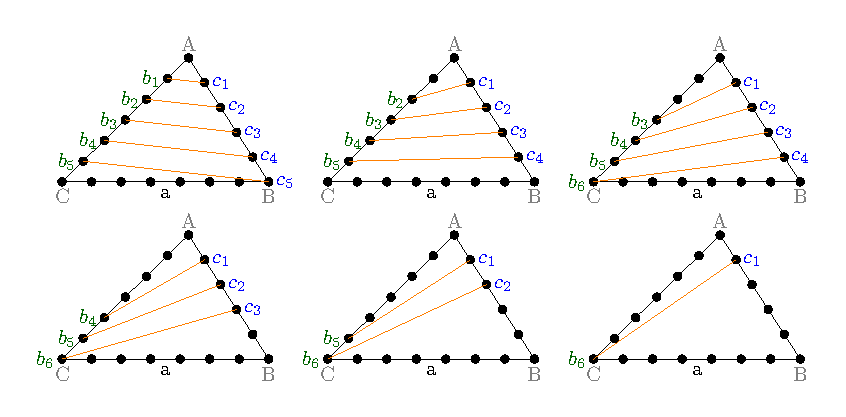
\includegraphics[scale=1]{t765bc}
\caption{Triangle $(7,6,5)$ $b_ic_j$ diagonals ($i \ge j$).}
\label{t765bc}
\end{figure}
Figure \ref{t765bc} show triangle $(7,6,5)$ diagonals $b_mc_n$ for vertex $A$.
The diagonals values are set in a first matrix with columns $b_1,...,b_6$ and rows $c_1,...,c_5$. Empty cells are repetitions.
\begin{equation}\label{eq:appendrow}
b_{1:6}c_{1:5} = \left(\begin{array}{cccccc}
\frac{2\sqrt{10}}{5} & \frac{\sqrt{105}}{5} & \frac{2\sqrt{55}}{5} & \frac{\sqrt{385}}{5} & 2\sqrt{6} & \frac{\sqrt{865}}{5} \\
& \frac{4\sqrt{10}}{5} & \frac{\sqrt{265}}{5} & \frac{2\sqrt{105}}{5} & 5 & \frac{4\sqrt{55}}{5} \\
& & \frac{6\sqrt{10}}{5} & \frac{\sqrt{505}}{5} & 2\sqrt{7} & \frac{3\sqrt{105}}{5} \\
& & & \frac{8\sqrt{10}}{5} & \sqrt{33} & \frac{2\sqrt{265}}{5} \\
& & & & 2\sqrt{10} & \\
\end{array}\right)
\end{equation}

\begin{figure}[htp]
\centering
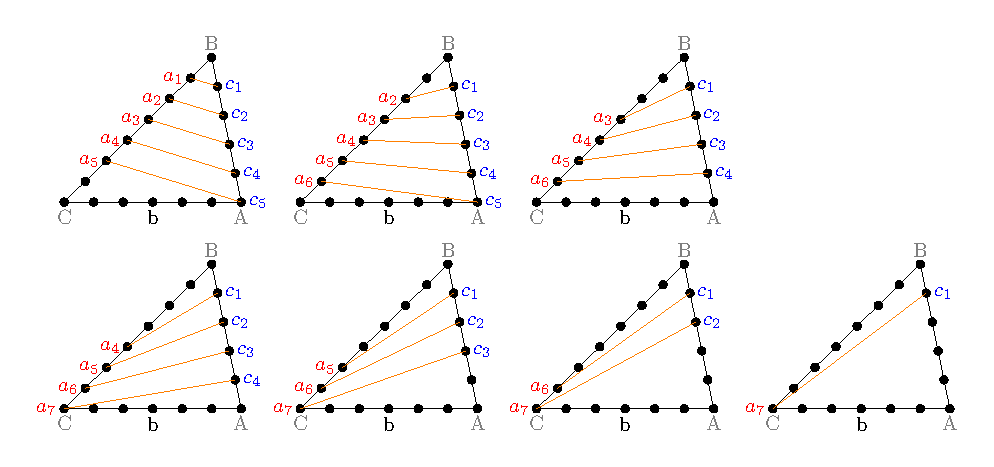
\includegraphics[scale=1]{t765ac}
\caption{Triangle $(7,6,5)$, $a_ic_j$ diagonals ($i \ge j$).}
\label{t765ac}
\end{figure}
Figure \ref{t765ac} show triangle $(7,6,5)$ diagonals $a_ic_j$ for vertex $B$. 
The diagonals are set in a second matrix with columns $a_1,...,a_7$ and rows $c_1,...,c_5$. Emtpy cells are repetitions.
Values at column 7 are repeated and already accounted in previous matrix.
\begin{equation}\label{eq:appendrow}
a_{1:7}c_{1:5}\left(\begin{array}{ccccccc}
\frac{4\sqrt{70}}{35} & \frac{3\sqrt{385}}{35} & \frac{2\sqrt{2065}}{35} & \frac{\sqrt{15505}}{35} & \frac{12\sqrt{7}}{7} & \frac{\sqrt{37345}}{35} & \frac{2\sqrt{265}}{5} \\
& \frac{8\sqrt{70}}{35} & \frac{\sqrt{7945}}{35} & \frac{6\sqrt{385}}{35} & \frac{\sqrt{889}}{7} & \frac{4\sqrt{2065}}{35} & \frac{3\sqrt{105}}{5} \\
& & \frac{12\sqrt{70}}{35} & \frac{\sqrt{14665}}{35} & \frac{2\sqrt{217}}{7} & \frac{9\sqrt{385}}{35} & \frac{4\sqrt{55}}{5} \\
& & & \frac{16\sqrt{70}}{35} & \frac{3\sqrt{105}}{7} & \frac{2\sqrt{7945}}{35} & \frac{\sqrt{865}}{5} \\
& & & & \frac{4\sqrt{70}}{7} & \frac{\sqrt{1393}}{7} & \\
\end{array}\right)
\end{equation}

\begin{figure}[htp]
\centering
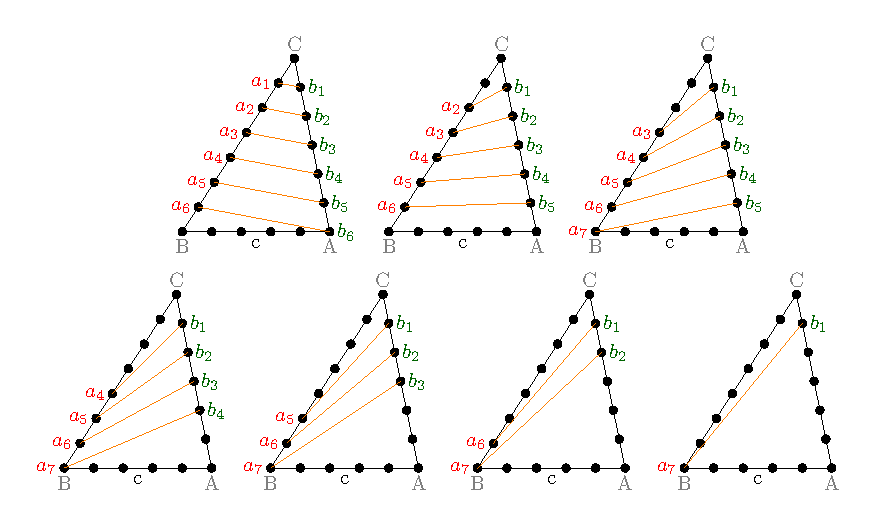
\includegraphics[scale=1]{t765ab}
\caption{Triangle $(7,6,5)$, $a_ib_j$ diagonals ($i \ge j$)}
\label{t765ab}
\end{figure}
Figure \ref{t765ab} show triangle $(7,6,5)$ diagonals $a_ib_j$ for vertex $C$.
The diagonals are set in a third matrix with columns $a_1,...,a_7$ and rows $b_1,...,b_6$. Empty cells are repetitions.
Values at columns 6 and 7 are repeated and already in previous matrices.
\begin{equation}\label{eq:appendrow}
a_{1:7}b_{1:6} = \left(\begin{array}{ccccccc}
\frac{2\sqrt{7}}{7} & \frac{\sqrt{105}}{7} & \frac{2\sqrt{70}}{7} & \frac{\sqrt{553}}{7} & \frac{2\sqrt{231}}{7} & \frac{\sqrt{1393}}{7} & 2\sqrt{10} \\
& \frac{4\sqrt{7}}{7} & \frac{\sqrt{217}}{7} & \frac{2\sqrt{105}}{7} & \frac{\sqrt{721}}{7} & \frac{4\sqrt{70}}{7} & \sqrt{33} \\
& & \frac{6\sqrt{7}}{7} & \frac{\sqrt{385}}{7} & \frac{2\sqrt{154}}{7} & \frac{3\sqrt{105}}{7} & 2\sqrt{7} \\
& & & \frac{8\sqrt{7}}{7} & \frac{\sqrt{609}}{7} & \frac{2\sqrt{217}}{7} & 5 \\
& & & & \frac{10\sqrt{7}}{7} & \frac{\sqrt{889}}{7} & 2\sqrt{6} \\
& & & & & \frac{12\sqrt{7}}{7} & \\
\end{array}\right)
\end{equation}
The values of the matrices are calculated with the code:
\texttt{github.com/heptagons/meccano/nest/t\_test.go TestT765diags}.

\section{Triangles$(\sqrt{\alpha},b,c)$}

Triangles$(\sqrt{\alpha},b,c)$ have three sides with lengths $a=\sqrt{\alpha}$, $b$ and $c$ where $\alpha, b, c \in \bbb N$
and $\alpha$ is square-free. We have:
\begin{align}
\sqrt{\alpha} &> b \ge c &\implies \alpha  > b^2 \ge c^2 \\
\sqrt{\alpha} &< b + c   &\implies \alpha < (b + c)^2
\end{align}
We calculate the triangle cosines. $\cos{A_{\alpha}}$ is rational and $\cos{B_{\alpha}}$ and $\cos{C_{\alpha}}$ are algebraic:
\begin{align}
\cos{A_{\alpha}} &= \frac{b^2 + c^2 - (\sqrt{\alpha})^2}{2bc} 
 = \frac{b^2 + c^2 - \alpha}{2bc} &\equiv \frac{\alpha_n}{\alpha_d} \in \bbb{Q} \\
\cos{B_{\alpha}} &= \frac{(\sqrt{\alpha})^2 + c^2 - b^2}{2\sqrt{\alpha}c}
 = \frac{(\alpha + c^2 - b^2)\sqrt{\alpha}}{2\alpha c} &\in \bbb{A} \\
\cos{C_{\alpha}} &= \frac{(\sqrt{\alpha})^2 + b^2 - c^2}{2\sqrt{\alpha}b}
 = \frac{(\alpha + b^2 - c^2)\sqrt{\alpha}}{2\alpha b} &\in \bbb{A} 
\end{align}

\subsection{Triangle $(\sqrt{\alpha},b,c)$ diagonals}

The only possible diagonals are for sides with integers points, that is segments $\overline{b_ic_j}$.
Using the law of cosines:
\begin{align}
\overline{b_ic_j} &= \sqrt{i^2 + j^2 - 2ij\cos{A_{\alpha}}} \nonumber\\
  &= \sqrt{i^2 + j^2 - 2ij\frac{\alpha_n}{\alpha_d}} \nonumber\\
  &= \frac{\sqrt{\alpha_d^2(i^2 + j^2)-2\alpha_nij}}{\alpha_d} &\in \bbb{A}
\end{align}
where $1 \le i \le b$, $1 \le j \le c$ and $i \ge j$.

\subsection{Example triangles$(2\sqrt{6},b,c)$}

In this case $\sqrt{\alpha} = 2\sqrt{6}$ so $\alpha = 24$.
Then sets $i = j = \{ 1,2,3,4 \}$ because sets $b^2 = c^2 = \{ 1,4,9,16\} < 24$.
We form a matrix with the values $(b+c)^2$ and satisfying $b \ge c$:
\begin {equation}\label{E:2}
(b_i + c_j)^2 =\bordermatrix{~ & b=1 & b=2 & b=3 & b=4 \cr
c=1 &  2 &  9 & 16 & 25 \cr    
c=2 & \times & 16 & 25 & 36 \cr    
c=3 & \times & \times & 36 & 49 \cr    
c=4 & \times & \times & \times & 64 \cr}
\end {equation}

Then we remove the cells that don't satisfy the condition $\alpha < (b+c)^2$:
\begin {equation}\label{E:3}
(b_m + c_n)^2 =\bordermatrix{~ & b=1 & b=2 & b=3 & b=4 \cr
c=1 & \times & \times & \times & 25 \cr    
c=2 & & \times & 25 & 36 \cr    
c=3 & & & 36 & 49 \cr    
c=4 & & & & 64 \cr}
\end {equation}

\begin{figure}[htp]
\centering
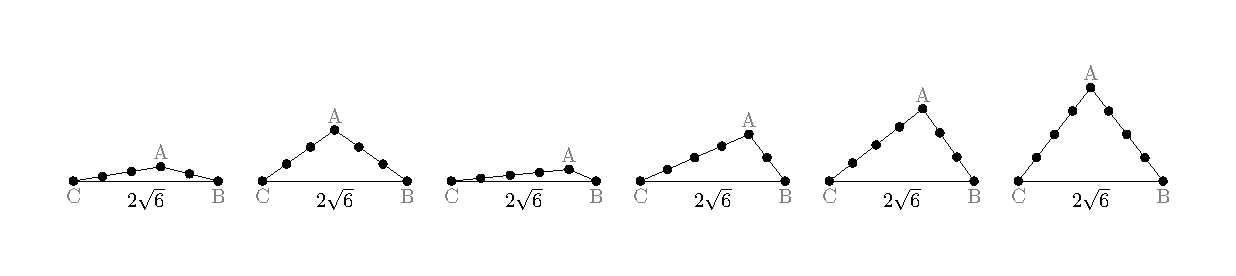
\includegraphics[scale=0.9]{tslurA}
\caption{All triangles with sides $a = 2\sqrt{6} > b \ge c$}
\label{tslurA}
\end{figure}
    
Each remaining cell in the matrix corresponds to a particular triangle:
\begin {equation}\label{E:4}
(2\sqrt{6},b,c) =\bordermatrix{~ & \cos{A_{\alpha}} & \cos{B_{\alpha}} & \cos{C_{\alpha}} \cr
(2\sqrt{6},3,2) & -\frac{11}{12} & \frac{19\sqrt{6}}{48} & \frac{29\sqrt{6}}{72} \cr
(2\sqrt{6},3,3) & -\frac{1}{3}   & \frac{\sqrt{6}}{3}    & \frac{\sqrt{6}}{3}    \cr
(2\sqrt{6},4,1) & -\frac{7}{8}   & \frac{3\sqrt{6}}{8}   & \frac{13\sqrt{6}}{32} \cr
(2\sqrt{6},4,2) & -\frac{1}{4}   & \frac{\sqrt{6}}{4}    & \frac{3\sqrt{6}}{8}   \cr
(2\sqrt{6},4,3) &  \frac{1}{24}  & \frac{17\sqrt{6}}{72} & \frac{31\sqrt{6}}{96} \cr
(2\sqrt{6},4,4) &  \frac{1}{4}   & \frac{\sqrt{6}}{4}    & \frac{\sqrt{6}}{4}    \cr}
\end{equation}

Figure \ref{tslurA} show the triangles $(2\sqrt{6},b,c)$. The cosines are calculated by code at:
\\\\
\texttt{github.com/heptagons/meccano/nest/t\_test.go TestTslursA}

\section{Triangles$(a,\sqrt{\beta},c)$}

Triangles$(a,\sqrt{\beta},c)$ have the three sides $a$, $b = \sqrt{\beta}$ and $c$ where $a, \beta, c \in \bbb N$ and $\beta$ is square-free.
We have:
\begin{align}
a &> \sqrt{\beta} > c &\implies a^2 > \beta > c^2 \\
a &< \sqrt{\beta} + c &\implies (a-c)^2 < \beta
\end{align}
We calculate the triangle cosines:
\begin{align}
\cos{A_{\beta}} &= \frac{(\sqrt{\beta})^2 + c^2 - a^2}{2\sqrt{\beta}c} = \frac{(\beta + c^2 - a^2)\sqrt{\beta}}{2\beta c} &\in \bbb{A} \\
\cos{B_{\beta}} &= \frac{a^2 + c^2 - (\sqrt{\beta})^2}{2ac} = \frac{a^2 + c^2 - \beta}{2ac} &\equiv \frac{\beta_n}{\beta_d} \in \bbb{Q} \\
\cos{C_{\beta}} &= \frac{a^2 + (\sqrt{\beta})^2 - c^2}{2a\sqrt{\beta}} = \frac{(a^2 + \beta - c^2)\sqrt{\beta}}{2a\beta} &\in \bbb{A} 
\end{align}

\subsection{Triangle $(a, \sqrt{\beta},c)$ diagonals}

The only possible diagonals are for sides with integers points, that is segments $\overline{a_ic_j}$.
Using the law of cosines:
\begin{align}
\overline{a_ic_j} &= \sqrt{i^2 + j^2 - 2ij\cos{B_{\beta}}}\\
  &= \sqrt{i^2 + j^2 - 2ij\frac{\beta_n}{\beta_d}}\\
  &= \frac{\sqrt{\beta_d^2(i^2 + j^2)-2\beta_nij}}{\beta_d} &\in \bbb{A}
\end{align}
where $1 \le i \le a$, $1 \le j \le c$ and $i \ge j$.

\subsection{Example triangles$(a,2\sqrt{6},c)$}

In this case $\sqrt{\beta} = 2\sqrt{6}$ so $\beta = 24$. 
Then $i = \{ 5,6,7,... \}$ because $a^2 = \{ 25,36,49,... \} > 24$ and
$j = \{ 1,2,3,4 \}$ because $c^2 = \{ 1,4,9,16\} < 24$.
We form a matrix with the values $(a-c)^2$:
\begin {equation}\label{E:11}
(a_i - c_j)^2 =\bordermatrix{~ & a=5 & a=6 & a=7 & a=8 & a=9 & ...\cr
c=1 & 16 & 25 & 36 & 49 & 64 & ...\cr    
c=2 &  9 & 16 & 25 & 36 & 49 & ...\cr    
c=3 &  4 &  9 & 16 & 25 & 36 & ...\cr    
c=4 &  1 &  4 &  9 & 16 & 25 & ...\cr}
\end {equation}

We remove cells which don't satisfy the condition $(a-c)^2 < \beta = 24$:
\begin {equation}\label{E:12}
(a_i - c_j)^2 =\bordermatrix{~ & a=5 & a=6 & a=7 & a=8 & a=9 & ...\cr
c=1 & 16 & \times & \times & \times & \times & ...\cr    
c=2 &  9 & 16 & \times & \times & \times & ...\cr    
c=3 &  4 &  9 & 16 & \times & \times & ...\cr    
c=4 &  1 &  4 &  9 & 16 & \times & ...\cr}
\end {equation}

\begin{figure}[htp]
\centering
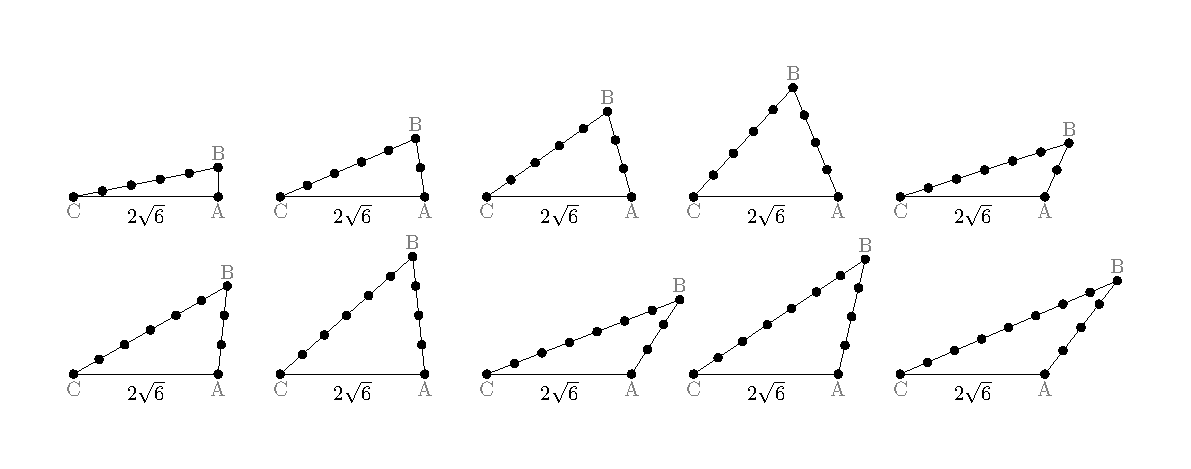
\includegraphics[scale=0.9]{tslurB}
\caption{All triangles with sides $a > b = 2\sqrt{6} > c$}
\label{tslurB}
\end{figure}

So we have ten triangles are valid:
\begin {equation}\label{E:13}
(a,2\sqrt{6},c) =\bordermatrix{~ & \cos{A_{\beta}} & \cos{B_{\beta}} & \cos{C_{\beta}} \cr
(5,2\sqrt{6},1) & 0         & \frac{1}{5} & \frac{2\sqrt{6}}{5} \cr
(5,2\sqrt{6},2) & \frac{\sqrt{6}}{16} & \frac{1}{4} & \frac{3\sqrt{6}}{8} \cr
(5,2\sqrt{6},3) & \frac{\sqrt{6}}{9} & \frac{1}{3} & \frac{\sqrt{6}}{3} \cr
(5,2\sqrt{6},4) & \frac{5\sqrt{6}}{32} & \frac{17}{40} & \frac{11\sqrt{6}}{40} \cr
(6,2\sqrt{6},2) & \frac{\sqrt{6}}{6} & \frac{2}{3} & \frac{7\sqrt{6}}{18} \cr
(6,2\sqrt{6},3) & \frac{\sqrt{6}}{24} & \frac{7}{12} & \frac{17\sqrt{6}}{48} \cr
(6,2\sqrt{6},4) & \frac{\sqrt{6}}{24} & \frac{7}{12} & \frac{11\sqrt{6}}{36} \cr
(7,2\sqrt{6},3) & -\frac{2\sqrt{6}}{9} & \frac{17}{21} & \frac{8\sqrt{6}}{21} \cr
(7,2\sqrt{6},4) & -\frac{3\sqrt{6}}{32} & \frac{41}{56} & \frac{19\sqrt{6}}{56} \cr
(8,2\sqrt{6},4) & \frac{\sqrt{6}}{4} & \frac{7}{8} & \frac{3\sqrt{6}}{8} \cr}
\end{equation}

Figure \ref{tslurB} show the triangles $(a,2\sqrt{6},c)$. The cosines are calculated by code at:
\\\\
\texttt{github.com/heptagons/meccano/nest/t\_test.go TestTslursB}


\section{Triangles$(a,b,\sqrt{\gamma})$}

Triangles$(a,b,\sqrt{\gamma})$ have three sides $a$, $b$, $\sqrt{\gamma}$ where $a, b, \gamma \in \bbb N$ and $\gamma$ is square-free.
We have:
\begin{align}
a &\ge b > \sqrt{\gamma} &\implies a^2 \ge b^2 > \gamma \\
a &< b + \sqrt{\gamma} &\implies (a-b)^2 < \gamma
\end{align}
We calculate the triangle cosines:
\begin{align}
\cos{A_{\gamma}} &= \frac{b^2 + \gamma - a^2}{2b\sqrt{\gamma}} = \frac{(b^2 + \gamma - a^2)\sqrt{\gamma}}{2b\gamma} &\in \bbb{A} \\
\cos{B_{\gamma}} &= \frac{a^2 + \gamma - b^2}{2a\sqrt{\gamma}} = \frac{(a^2 + \gamma - b^2)\sqrt{\gamma}}{2a\gamma} &\in \bbb{A} \\
\cos{C_{\gamma}} &= \frac{a^2 + b^2 - (\sqrt{\gamma})^2}{2ab} = \frac{a^2 + b^2 - \gamma}{2ab} &\equiv \frac{\gamma_n}{\gamma_d} \in \bbb{Q} 
\end{align}

\subsection{Triangle $(a, b, \sqrt{\gamma})$ diagonals}

The only possible diagonals are for sides with integers, that is $\overline{a_mb_n}$. Using the law of cosines:
\begin{align}
\overline{a_mb_n} &= \sqrt{m^2 + n^2 - 2mn\cos{C}}\\
  &= \sqrt{m^2 + n^2 - 2mn\frac{a^2 + b^2 - \gamma}{2ab}}\\
  &= \frac{\sqrt{a^2b^2(m^2 + n^2)-acmn(a^2 + b^2 - \gamma)}}{ab} &\in \bbb{A}
\end{align}
where $1 \le m < a$, $1 \le n < b$ and $m \ge n$.

\subsection{Example triangles$(a,b,2\sqrt{6})$}

In this case $\sqrt{\gamma} = 2\sqrt{6}$ so $\gamma = 24$. 
We form a matrix with with the values $(a-b)^2$ satisfying the condition $a^2 \ge b^2 > \gamma$:
\begin {equation}\label{E:21}
(a_m - b_n)^2 =\bordermatrix{~ & a=5 & a=6 & a=7 & a=8 & a=9 & a=10 & a=11 & a=12 & \hdots\cr
b=5  & 0 & 1 & 4 &  9 & 16 & 25 & 36 & 49 & \hdots \cr    
b=6  &   & 0 & 1 &  4 &  9 & 16 & 25 & 36 & \hdots \cr    
b=7  &   &   & 0 &  1 &  4 &  9 & 16 & 25 & \hdots \cr    
b=8  &   &   &   &  0 &  1 &  4 &  9 & 16 & \hdots \cr    
b=9  &   &   &   &    &  0 &  1 &  4 &  9 & \hdots \cr    
b=10 &   &   &   &    &    &  0 &  1 &  4 & \hdots \cr    
 &  &  &  &  &  & \vdots & \vdots & \vdots & \ddots \cr}
\end {equation}

We remove cells except those satisfying the condition $(a-b)^2 < \gamma$:
\begin {equation}\label{E:21}
(a_m - b_n)^2 =\bordermatrix{~ & a=5 & a=6 & a=7 & a=8 & a=9 & a=10 & a=11 & a=12 & \hdots\cr
b=5  & 0 & 1 & 4 &  9 & 16 & \times & \times & \times & \hdots \cr    
b=6  &   & 0 & 1 &  4 &  9 & 16 & \times & \times & \hdots \cr    
b=7  &   &   & 0 &  1 &  4 &  9 & 16 & \times & \hdots \cr    
b=8  &   &   &   &  0 &  1 &  4 &  9 & 16 & \hdots \cr    
b=9  &   &   &   &    &  0 &  1 &  4 &  9 & \hdots \cr    
b=10 &   &   &   &    &    &  0 &  1 &  4 & \hdots \cr    
 &  &  &  &  &  & \vdots & \vdots & \vdots & \ddots \cr}
\end {equation}

\begin{figure}[htp]
\centering
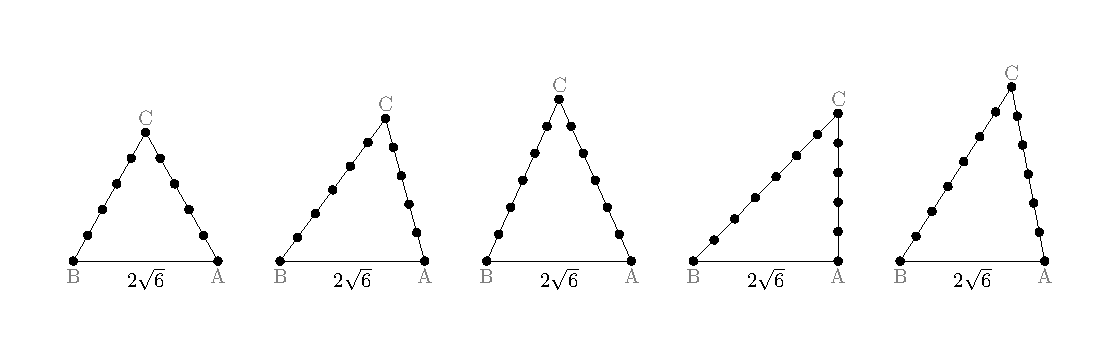
\includegraphics[scale=0.9]{tslurC}
\caption{Some triangles with sides $a \ge b > c = 2\sqrt{6}$}
\label{tslurC}
\end{figure}

So we found that infinite triangles are valid, the smaller ones are:
\begin {equation}\label{E:4}
(a,b,2\sqrt{6}) =\bordermatrix{~ & \cos{A} & \cos{B} & \cos{C} \cr
(5,5,2\sqrt{6}) & \frac{\sqrt{6}}{5} & \frac{\sqrt{6}}{5} & \frac{13}{25} \cr
(6,5,2\sqrt{6}) & \frac{13\sqrt{6}}{120} & \frac{35\sqrt{6}}{144} & \frac{37}{60} \cr
(6,6,2\sqrt{6}) & \frac{\sqrt{6}}{6} & \frac{\sqrt{6}}{6} & \frac{2}{3} \cr
(7,5,2\sqrt{6}) & 0 & \frac{2\sqrt{6}}{7} & \frac{5}{7} \cr
(7,6,2\sqrt{6}) & \frac{11\sqrt{6}}{144} & \frac{37\sqrt{6}}{168} & \frac{61}{84} \cr
(7,7,2\sqrt{6}) & \frac{\sqrt{6}}{7} & \frac{\sqrt{6}}{7} & \frac{37}{49} \cr
\hdots & \hdots & \hdots & \hdots \cr}
\end{equation}

Figure \ref{tslurC} show some triangles $(a,b,2\sqrt{6})$. The cosines are calculated by code at:
\\\\
\texttt{github.com/heptagons/meccano/nest/t\_test.go TestTslursC}

\section{Triangles pairs}

We can attach two triangles to share a common side and vertex to get more angles and diagonals.

\subsection{Triangles pairs rational cosines angles}
When we sum two angles $Z = X+Y$, where $\cos{X} \equiv x_N / x_D$ and $\cos{Y} \equiv y_N / y_D$ we have:
\begin{align}
\cos{Z} &= \cos{X}\cos{Y} - \sin{X}\sin{Y}\\
 &= \frac{x_N}{x_D} \times \frac{y_N}{y_D} - \frac{\sqrt{x_S}}{x_D} \times \frac{\sqrt{y_S}}{y_D}\\
 &= \frac{x_Ny_N - \sqrt{x_Sy_S}}{x_Dy_D}
\end{align}

\subsubsection{Triangles pairs angles}

Adding the angles of Triangles from $(1,1,1)$ to $(3,3,2)$ we get some sums. The values are calculated with code at:
\\\\
\texttt{github.com/heptagons/meccano/nest/t\_test.go TestTCosAplusB}

\begin{longtable}{ | p{1cm}| *{15}{c|} }
\hline
Pair & $vertex_X$ & $vertex_Y$ & $\cos(X+Y)$ \\
\hline\endhead
\hline
Pair & $vertex_X$ & $vertex_Y$ & $\cos(X+Y)$ \\
\hline\endfoot
1 & (1,1,1)[A] & (1,1,1)[A] & $-\frac{1}{2}$\\ %-1/2
2 & (2,2,1)[A] & (1,1,1)[A] & $\frac{1-3\sqrt{5}}{8}$\\ %(1-3√5)/8
3 & (2,2,1)[C] & (1,1,1)[A] & $\frac{7-3\sqrt{5}}{16}$\\ %(7-3√5)/16
4 & (2,2,1)[A] & (2,2,1)[A] & $-\frac{7}{8}$\\ %-7/8
5 & (2,2,1)[A] & (2,2,1)[C] & $-\frac{1}{4}$\\ %-1/4
6 & (2,2,1)[C] & (2,2,1)[C] & $\frac{17}{32}$\\ %17/32
7 & (3,2,2)[A] & (1,1,1)[A] & $-\frac{1+3\sqrt{21}}{16}$\\ %(-1-3√21)/16
8 & (3,2,2)[B] & (1,1,1)[A] & $\frac{3-\sqrt{21}}{8}$\\ %(3√21)/8
9 & (3,2,2)[A] & (2,2,1)[A] & $-\frac{1+3\sqrt{105}}{32}$\\ %(-1-3√105)/32
10 & (3,2,2)[A] & (2,2,1)[C] & $-\frac{7+3\sqrt{105}}{64}$\\ %(-7-3√105)/64
11 & (3,2,2)[B] & (2,2,1)[A] & $\frac{3-\sqrt{105}}{16}$\\ %(3√105)/16
12 & (3,2,2)[B] & (2,2,1)[C] & $\frac{21-\sqrt{105}}{32}$\\ %(21√105)/32
13 & (3,2,2)[A] & (3,2,2)[A] & $-\frac{31}{32}$\\ %-31/32
14 & (3,2,2)[A] & (3,2,2)[B] & $-\frac{3}{4}$\\ %-3/4
15 & (3,2,2)[B] & (3,2,2)[B] & $\frac{1}{8}$\\ %1/8
16 & (3,3,1)[A] & (1,1,1)[A] & $\frac{1-\sqrt{105}}{12}$\\ %(1√105)/12
17 & (3,3,1)[C] & (1,1,1)[A] & $\frac{17-\sqrt{105}}{36}$\\ %(17√105)/36
18 & (3,3,1)[A] & (2,2,1)[A] & $\frac{1-5\sqrt{21}}{24}$\\ %(1-5√21)/24
19 & (3,3,1)[A] & (2,2,1)[C] & $\frac{7-5\sqrt{21}}{48}$\\ %(7-5√21)/48
20 & (3,3,1)[C] & (2,2,1)[A] & $\frac{17-5\sqrt{21}}{72}$\\ %(17-5√21)/72
21 & (3,3,1)[C] & (2,2,1)[C] & $\frac{119-5\sqrt{21}}{144}$\\ %(119-5√21)/144
22 & (3,3,1)[A] & (3,2,2)[A] & $-\frac{1+21\sqrt{5}}{48}$\\ %(-1-21√5)/48
23 & (3,3,1)[A] & (3,2,2)[B] & $\frac{3-7\sqrt{5}}{24}$\\ %(3-7√5)/24
24 & (3,3,1)[C] & (3,2,2)[A] & $-\frac{17+21\sqrt{5}}{144}$\\ %(-17-21√5)/144
25 & (3,3,1)[C] & (3,2,2)[B] & $\frac{51-7\sqrt{5}}{72}$\\ %(51-7√5)/72
26 & (3,3,1)[A] & (3,3,1)[A] & $-\frac{17}{18}$\\ %-17/18
27 & (3,3,1)[A] & (3,3,1)[C] & $-\frac{1}{6}$\\ %-1/6
28 & (3,3,1)[C] & (3,3,1)[C] & $\frac{127}{162}$\\ %127/162
29 & (3,3,2)[A] & (1,1,1)[A] & $\frac{1-2\sqrt{6}}{6}$\\ %(1-2√6)/6
30 & (3,3,2)[C] & (1,1,1)[A] & $\frac{7-4\sqrt{6}}{18}$\\ %(7-4√6)/18
31 & (3,3,2)[A] & (2,2,1)[A] & $\frac{1-2\sqrt{30}}{12}$\\ %(1-2√30)/12
32 & (3,3,2)[A] & (2,2,1)[C] & $\frac{7-2\sqrt{30}}{24}$\\ %(7-2√30)/24
33 & (3,3,2)[C] & (2,2,1)[A] & $\frac{7-4\sqrt{30}}{36}$\\ %(7-4√30)/36
34 & (3,3,2)[C] & (2,2,1)[C] & $\frac{49-4\sqrt{30}}{72}$\\ %(49-4√30)/72
35 & (3,3,2)[A] & (3,2,2)[A] & $-\frac{1+6\sqrt{14}}{24}$\\ %(-1-6√14)/24
36 & (3,3,2)[A] & (3,2,2)[B] & $\frac{3-2\sqrt{14}}{12}$\\ %(3-2√14)/12
37 & (3,3,2)[C] & (3,2,2)[A] & $-\frac{7+12\sqrt{14}}{72}$\\ %(-7-12√14)/72
38 & (3,3,2)[C] & (3,2,2)[B] & $\frac{21-4\sqrt{14}}{36}$\\ %(21-4√14)/36
39 & (3,3,2)[A] & (3,3,1)[A] & $\frac{1-2\sqrt{70}}{18}$\\ %(1-2√70)/18
40 & (3,3,2)[A] & (3,3,1)[C] & $\frac{17-2\sqrt{70}}{54}$\\ %(17-2√70)/54
41 & (3,3,2)[C] & (3,3,1)[A] & $\frac{7-4\sqrt{70}}{54}$\\ %(7-4√70)/54
42 & (3,3,2)[C] & (3,3,1)[C] & $\frac{119-4\sqrt{70}}{162}$\\ %(119-4√70)/162
43 & (3,3,2)[A] & (3,3,2)[A] & $-\frac{7}{9}$\\ %-7/9
44 & (3,3,2)[A] & (3,3,2)[C] & $-\frac{1}{3}$\\ %-1/3
45 & (3,3,2)[C] & (3,3,2)[C] & $\frac{17}{81}$\\ %17/81
\end{longtable}

We can also test more triangles and filter, for example, the cosines to contain term $\sqrt{5}$:
\begin{longtable}{ | p{1cm}| *{15}{c|} }
\hline
Pair & $vertex_X$ & $vertex_Y$ & $\cos(X+Y)$ \\
\hline\endhead
\hline
Pair & $vertex_X$ & $vertex_Y$ & $\cos(X+Y)$ \\
\hline\endfoot
1 & (2,2,1)[A] & (1,1,1)[A] & $\frac{1-3\sqrt{5}}{8}$\\ %(1-3√5)/8
2 & (2,2,1)[C] & (1,1,1)[A] & $\frac{7-3\sqrt{5}}{16}$\\ %(7-3√5)/16
3 & (3,3,1)[A] & (3,2,2)[A] & $-\frac{1+21\sqrt{5}}{48}$\\ %(-1-21√5)/48
4 & (3,3,1)[A] & (3,2,2)[B] & $\frac{3-7\sqrt{5}}{24}$\\ %(3-7√5)/24
5 & (3,3,1)[C] & (3,2,2)[A] & $-\frac{17+21\sqrt{5}}{144}$\\ %(-17-21√5)/144
6 & (3,3,1)[C] & (3,2,2)[B] & $\frac{51-7\sqrt{5}}{72}$\\ %(51-7√5)/72
7 & (4,3,2)[A] & (1,1,1)[A] & $-\frac{1+3\sqrt{5}}{8}$\\ %(-1-3√5)/8
8 & (4,3,2)[B] & (1,1,1)[A] & $\frac{11-9\sqrt{5}}{32}$\\ %(11-9√5)/32
9 & (4,4,1)[A] & (3,3,1)[A] & $\frac{1-21\sqrt{5}}{48}$\\ %(1-21√5)/48
10 & (4,4,1)[A] & (3,3,1)[C] & $\frac{17-21\sqrt{5}}{144}$\\ %(17-21√5)/144
11 & (4,4,1)[C] & (3,3,1)[A] & $\frac{31-21\sqrt{5}}{192}$\\ %(31-21√5)/192
12 & (4,4,1)[C] & (3,3,1)[C] & $\frac{527-21\sqrt{5}}{576}$\\ %(527-21√5)/576
13 & (5,3,3)[A] & (4,4,3)[A] & $-\frac{21+55\sqrt{5}}{144}$\\ %(-21-55√5)/144
14 & (5,3,3)[A] & (4,4,3)[C] & $-\frac{161+165\sqrt{5}}{576}$\\ %(-161-165√5)/576
15 & (5,3,3)[B] & (4,4,3)[A] & $\frac{15-11\sqrt{5}}{48}$\\ %(15-11√5)/48
16 & (5,3,3)[B] & (4,4,3)[C] & $\frac{115-33\sqrt{5}}{192}$\\ %(115-33√5)/192
17 & (5,4,3)[A] & (4,3,3)[A] & $\frac{-4\sqrt{5}}{9}$\\ %-4√5/9
18 & (5,4,3)[A] & (4,3,3)[B] & $\frac{-\sqrt{5}}{3}$\\ %√5/3
19 & (5,4,3)[B] & (4,3,3)[A] & $\frac{3-16\sqrt{5}}{45}$\\ %(3-16√5)/45
20 & (5,4,3)[B] & (4,3,3)[B] & $\frac{6-4\sqrt{5}}{15}$\\ %(6-4√5)/15
21 & (5,4,3)[C] & (4,3,3)[A] & $\frac{4-12\sqrt{5}}{45}$\\ %(4-12√5)/45
22 & (5,4,3)[C] & (4,3,3)[B] & $\frac{8-3\sqrt{5}}{15}$\\ %(8-3√5)/15
23 & (5,5,1)[A] & (4,4,3)[A] & $\frac{3-33\sqrt{5}}{80}$\\ %(3-33√5)/80
24 & (5,5,1)[A] & (4,4,3)[C] & $\frac{23-99\sqrt{5}}{320}$\\ %(23-99√5)/320
25 & (5,5,1)[C] & (4,4,3)[A] & $\frac{147-33\sqrt{5}}{400}$\\ %(147-33√5)/400
26 & (5,5,1)[C] & (4,4,3)[C] & $\frac{1127-99\sqrt{5}}{1600}$\\ %(1127-99√5)/1600
\end{longtable}

\subsection{Triangles pairs diagonals}


So we can calculate new diagonals from one triangle side to another triangle side:
\begin{align}
\delta &= \sqrt{m^2 + n^2 - 2mn\cos{Z}}\\
 &= \sqrt{m^2 + n^2 - 2mn\frac{b_1+c_1\sqrt{d_1}}{a_1}}\\
 &= \frac{\sqrt{a_1^2(m^2 + n^2) - 2mn(b_1 + c_1\sqrt{d_1})}}{a_1}\\
 &= \frac{\sqrt{a_1^2(m^2 + n^2) - 2b_1mn - 2c_1mn\sqrt{d_1} }}{a_1} &\equiv \frac{b_2 + c_2\sqrt{d_2 + e_2\sqrt{f_2}}}{a_2}
\end{align}

\subsection{Triangles pairs surds angles}

When we sum two algebraic angles $W = U+V$ when $\cos{U} = \sqrt{u_n}/u_d$ and $\cos{V} = \sqrt{v_n}/v_d$ we have:
\begin{align}
\cos{W} &= \cos{U}\cos{V} - \sin{U}\sin{V}\\
 &= \cos{U}\cos{V} - \sqrt{1 - \cos^2{U}}\sqrt{1 - \cos^2{V}}\\
 &= \frac{\sqrt{u_nv_n}}{u_dv_d} - \sqrt{\frac{u_d^2 - u_n}{u_d^2}} \sqrt{\frac{v_d^2 - v_n}{v_d^2}}\\
 &= \frac{\sqrt{u_nv_n} - \sqrt{(u_d^2 - u_n)(v_d^2 - v_n)} }{u_dv_d}
\end{align}

\section{Triangle triplets}

We can attach three triangles to share a common vertex and two sides.

\subsection{Triple angles $2A+D$ and $A+2D$}

Lets add three angles, two angles $A$ from a pair of triangles $(a,b,c)$ and one angle $D$ from single triangle $(d,e,f)$.
For triangle $(a,b,c)$ and using $\cos{A}$ and $\sin{A}$ from equations \ref{Eq:cosABC} and \ref{Eq:sinABC} we have:
\begin{align}
\cos{(2A)} &= 2\cos^2{A} - 1 = 2\frac{a_N^2}{a_D^2} - 1 &= \frac{2a_N^2 - a_D^2}{a_D^2}\\
\sin{(2A)} &= 2\sin{A}\cos{A} &= \frac{2a_N\sqrt{a_D^2 - a_N^2}}{a_D^2}
\end{align}

As with equations \ref{Eq:cosABC} and \ref{Eq:sinABC} lets define cosines and sines of triangle $(d,e,f)$:

\begin{equation}\label{Eq:cossinDEF}
\left({\begin{array}{c c} {\cos} & {\sin}\end{array}}\right)
\left({\begin{array}{c} D\\ E\\ F\\ \end{array}}\right)
= \left({\begin{array}{c c}
\dfrac{d_N}{d_D} & \dfrac{\sqrt{d_D^2 - d_N^2}}{d_D}\\[10pt]
\dfrac{e_N}{e_D} & \dfrac{\sqrt{e_D^2 - e_N^2}}{e_D}\\[10pt]
\dfrac{f_N}{f_D} & \dfrac{\sqrt{f_D^2 - f_N^2}}{f_D}\\[10pt]
\end{array}}\right)
\end{equation}

Using $\cos{(2A)}$, $\sin{(2A)}$, $\cos{D}$ and $\sin{D}$ we have:
\begin{align}
\cos{(2A+D)} &= \cos{(2A)}\cos{D} - \sin{(2A)}\sin{D}\\
 &= \frac{(2a_N^2 - a_D^2)d_N - 2a_N\sqrt{(a_D^2 - a_N^2)(d_D^2 - d_N^2)}}{a_D^2d_D}
\end{align}

\begin{longtable}{ | p{1cm}| *{15}{c|} }
\caption{Pair of triangles $(X_{ABC})$ and $(Y_{ABC})$ adding three angles 
in two different forms $(2X+Y)$ and $(X+2Y)$.}\\
\hline
Pair & $X = A \lor B \lor C$ & $Y = A \lor B \lor C$ & $\cos(2X+Y)$ & $\cos(X+2Y)$ \\
\hline\endhead
\hline\endfoot
1 & (1,1,1)[A] & (1,1,1)[A] & $\frac{1}{2}$ & $\frac{1}{2}$\\
2 & (2,2,1)[A] & (1,1,1)[A] & $-\frac{7-3\sqrt{5}}{16}$ & $-\frac{1-3\sqrt{5}}{8}$\\
3 & (2,2,1)[C] & (1,1,1)[A] & $\frac{17+21\sqrt{5}}{64}$ & $-\frac{7-3\sqrt{5}}{16}$\\
4 & (2,2,1)[A] & (2,2,1)[A] & $\frac{1}{4}$ & $\frac{1}{4}$\\
5 & (2,2,1)[A] & (2,2,1)[C] & $-\frac{17}{32}$ & $\frac{61}{64}$\\
6 & (2,2,1)[C] & (2,2,1)[A] & $\frac{61}{64}$ & $-\frac{17}{32}$\\
7 & (2,2,1)[C] & (2,2,1)[C] & $\frac{7}{8}$ & $\frac{7}{8}$\\
8 & (3,2,2)[A] & (1,1,1)[A] & $-\frac{31+3\sqrt{21}}{64}$ & $\frac{1+3\sqrt{21}}{16}$\\
9 & (3,2,2)[B] & (1,1,1)[A] & $\frac{1+3\sqrt{21}}{16}$ & $-\frac{3-\sqrt{21}}{8}$\\
10 & (3,2,2)[A] & (2,2,1)[A] & $-\frac{31+3\sqrt{105}}{128}$ & $\frac{7+3\sqrt{105}}{64}$\\
11 & (3,2,2)[A] & (2,2,1)[C] & $-\frac{217+3\sqrt{105}}{256}$ & $-\frac{17-21\sqrt{105}}{256}$\\
12 & (3,2,2)[B] & (2,2,1)[A] & $\frac{1+3\sqrt{105}}{32}$ & $-\frac{21-\sqrt{105}}{32}$\\
13 & (3,2,2)[B] & (2,2,1)[C] & $\frac{7+3\sqrt{105}}{64}$ & $\frac{51+7\sqrt{105}}{128}$\\
14 & (3,2,2)[A] & (3,2,2)[A] & $-\frac{1}{8}$ & $-\frac{1}{8}$\\
15 & (3,2,2)[A] & (3,2,2)[B] & $-\frac{57}{64}$ & $\frac{31}{32}$\\
16 & (3,2,2)[B] & (3,2,2)[A] & $\frac{31}{32}$ & $-\frac{57}{64}$\\
17 & (3,2,2)[B] & (3,2,2)[B] & $\frac{3}{4}$ & $\frac{3}{4}$\\
18 & (3,3,1)[A] & (1,1,1)[A] & $-\frac{17-\sqrt{105}}{36}$ & $-\frac{1-\sqrt{105}}{12}$\\
19 & (3,3,1)[C] & (1,1,1)[A] & $\frac{127+17\sqrt{105}}{324}$ & $-\frac{17-\sqrt{105}}{36}$\\
20 & (3,3,1)[A] & (2,2,1)[A] & $-\frac{17-5\sqrt{21}}{72}$ & $-\frac{7-5\sqrt{21}}{48}$\\
21 & (3,3,1)[A] & (2,2,1)[C] & $-\frac{119-5\sqrt{21}}{144}$ & $\frac{17+35\sqrt{21}}{192}$\\
22 & (3,3,1)[C] & (2,2,1)[A] & $\frac{127+85\sqrt{21}}{648}$ & $-\frac{119-5\sqrt{21}}{144}$\\
23 & (3,3,1)[C] & (2,2,1)[C] & $\frac{889+85\sqrt{21}}{1296}$ & $\frac{289+35\sqrt{21}}{576}$\\
24 & (3,3,1)[A] & (3,2,2)[A] & $\frac{17+21\sqrt{5}}{144}$ & $-\frac{31+21\sqrt{5}}{192}$\\
25 & (3,3,1)[A] & (3,2,2)[B] & $-\frac{51-7\sqrt{5}}{72}$ & $\frac{1+21\sqrt{5}}{48}$\\
26 & (3,3,1)[C] & (3,2,2)[A] & $-\frac{127-357\sqrt{5}}{1296}$ & $-\frac{527+21\sqrt{5}}{576}$\\
27 & (3,3,1)[C] & (3,2,2)[B] & $\frac{381+119\sqrt{5}}{648}$ & $\frac{17+21\sqrt{5}}{144}$\\
28 & (3,3,1)[A] & (3,3,1)[A] & $\frac{1}{6}$ & $\frac{1}{6}$\\
29 & (3,3,1)[A] & (3,3,1)[C] & $-\frac{127}{162}$ & $\frac{361}{486}$\\
30 & (3,3,1)[C] & (3,3,1)[A] & $\frac{361}{486}$ & $-\frac{127}{162}$\\
31 & (3,3,1)[C] & (3,3,1)[C] & $\frac{17}{18}$ & $\frac{17}{18}$\\
32 & (3,3,2)[A] & (1,1,1)[A] & $-\frac{7-4\sqrt{6}}{18}$ & $-\frac{1-2\sqrt{6}}{6}$\\
33 & (3,3,2)[C] & (1,1,1)[A] & $\frac{17+56\sqrt{6}}{162}$ & $-\frac{7-4\sqrt{6}}{18}$\\
34 & (3,3,2)[A] & (2,2,1)[A] & $-\frac{7-4\sqrt{30}}{36}$ & $-\frac{7-2\sqrt{30}}{24}$\\
35 & (3,3,2)[A] & (2,2,1)[C] & $-\frac{49-4\sqrt{30}}{72}$ & $\frac{17+14\sqrt{30}}{96}$\\
36 & (3,3,2)[C] & (2,2,1)[A] & $\frac{17+56\sqrt{30}}{324}$ & $-\frac{49-4\sqrt{30}}{72}$\\
37 & (3,3,2)[C] & (2,2,1)[C] & $\frac{119+56\sqrt{30}}{648}$ & $\frac{119+28\sqrt{30}}{288}$\\
38 & (3,3,2)[A] & (3,2,2)[A] & $\frac{7+12\sqrt{14}}{72}$ & $-\frac{31+6\sqrt{14}}{96}$\\
39 & (3,3,2)[A] & (3,2,2)[B] & $-\frac{21-4\sqrt{14}}{36}$ & $\frac{1+6\sqrt{14}}{24}$\\
40 & (3,3,2)[C] & (3,2,2)[A] & $-\frac{17-168\sqrt{14}}{648}$ & $-\frac{217+12\sqrt{14}}{288}$\\
41 & (3,3,2)[C] & (3,2,2)[B] & $\frac{51+56\sqrt{14}}{324}$ & $\frac{7+12\sqrt{14}}{72}$\\
42 & (3,3,2)[A] & (3,3,1)[A] & $-\frac{7-4\sqrt{70}}{54}$ & $-\frac{17-2\sqrt{70}}{54}$\\
43 & (3,3,2)[A] & (3,3,1)[C] & $-\frac{119-4\sqrt{70}}{162}$ & $\frac{127+34\sqrt{70}}{486}$\\
44 & (3,3,2)[C] & (3,3,1)[A] & $\frac{17+56\sqrt{70}}{486}$ & $-\frac{119-4\sqrt{70}}{162}$\\
45 & (3,3,2)[C] & (3,3,1)[C] & $\frac{289+56\sqrt{70}}{1458}$ & $\frac{889+68\sqrt{70}}{1458}$\\
46 & (3,3,2)[A] & (3,3,2)[A] & $\frac{1}{3}$ & $\frac{1}{3}$\\
47 & (3,3,2)[A] & (3,3,2)[C] & $-\frac{17}{81}$ & $\frac{241}{243}$\\
48 & (3,3,2)[C] & (3,3,2)[A] & $\frac{241}{243}$ & $-\frac{17}{81}$\\
49 & (3,3,2)[C] & (3,3,2)[C] & $\frac{7}{9}$ & $\frac{7}{9}$\\
\end{longtable}
Data from:\texttt{github.com/heptagons/meccano/nest/t\_test.go TestTCos2AplusB}

\subsection{Triple angles $Z = A+D+G$}

\begin{align}
\cos{(A+D)} &= \cos{A}\cos{D} - \sin{A}\sin{D} \nonumber\\
 &= \frac{a_nd_n - \sqrt{a_sd_s}}{a_dd_d}\\
\sin{(A+D)} &= \sin{A}\cos{D} + \cos{A}\sin{D} \nonumber\\
 &= \frac{d_n\sqrt{a_s} + a_n\sqrt{d_s}}{a_dd_d}\\
\cos{(A+D+G)} &= \cos{(A+D)}\cos{G} - \sin{(A+D)}\sin{G} \nonumber\\
 &= \frac{a_nd_ng_n - g_n\sqrt{a_sd_s}}{a_dd_dg_d}
 -\frac{d_n\sqrt{a_sg_s} + a_n\sqrt{d_sg_s}}{a_dd_dg_d} \nonumber\\
 &= \frac{a_nd_ng_n - g_n\sqrt{a_sd_s} - d_n\sqrt{a_sg_s} - a_n\sqrt{d_sg_s}}{a_dd_dg_d}
\end{align}

\begin{longtable}{ | p{1cm}| *{15}{c|} }
\caption{Pair of triangles $(X_{ABC})$ and $(Y_{ABC})$ adding three angles 
in two different forms $(2X+Y)$ and $(X+2Y)$.}\\
\hline
Pair & $X = A \lor B \lor C$ & $Y = A \lor B \lor C$ & $Z = A \lor B \lor C$ & $\cos(X+Y+Z)$ \\
\hline\endhead
\hline\endfoot
\end{longtable}
Data from:\texttt{github.com/heptagons/meccano/nest/t\_test.go TestTCosAplusBplusC}




\end{document}